% Created 2017-04-07 Sex 17:55
\documentclass{article}
\usepackage[top=1in, bottom=1.in, left=2in, right=2in]{geometry}
  

\usepackage[utf8]{inputenc}
\usepackage[T1]{fontenc}
\usepackage{fixltx2e}
\usepackage{graphicx}
\usepackage{longtable}
\usepackage{float}
\usepackage{wrapfig}
\usepackage{rotating}
\usepackage[normalem]{ulem}
\usepackage{amsmath}
\usepackage{textcomp}
\usepackage{marvosym}
\usepackage{wasysym}
\usepackage{amssymb}
\usepackage{hyperref}
\tolerance=1000
\author{Arthur Colombini Gusmão}
\date{\today}
\title{relatorio\_final}
\hypersetup{
  pdfkeywords={},
  pdfsubject={},
  pdfcreator={Emacs 24.5.1 (Org mode 8.2.10)}}
\begin{document}

\maketitle

\section{Without missing data, learn the Bayesian Network parameters using SamIam}
\label{sec-1}
In the last homework, we selected 5 features that we thought most relevant for finding out if
the person earns more than 50k dollars a year, they were:
\begin{itemize}
\item age
\item workclass
\item education-num
\item occupation
\item sex
\end{itemize}

We also converted all features to binary, including the label, so that we ended up with the
following rule:
\begin{center}
\begin{tabular}{lll}
\hline
\textbf{FEATURE} & \textbf{STATE 0} & \textbf{STATE 1}\\
\hline
\textbf{age} & between 17 and 25 or & between 26 and 65\\
 & greater than 65 & \\
\hline
\textbf{workclass} & Never-worked, Private, & Federal-gov, Local-gov,\\
 & Self-emp-not-inc, & Self-emp-inc, State-gov\\
 & Without pay & \\
\hline
\textbf{education-num} & <= 9 & >= 10 (some college or greater)\\
\hline
\textbf{occupation} & All other not included & Exec-managerial, Prof-specialty,\\
 & in state 1 & Protective-serv, Tech-support\\
\hline
\textbf{sex} & Female & Male\\
\hline
\textbf{label} & <=50K & >50K\\
\hline
\end{tabular}
\end{center}

Our initial guess of the structure of the network was the following (which corresponds to a
Naive Bayes approach):

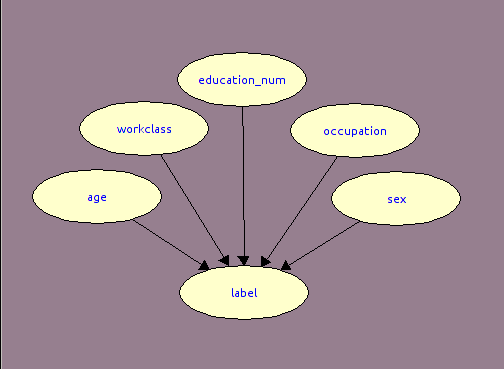
\includegraphics[width=.9\linewidth]{./img/bayes_net.png}
\\

Now, we are going to stick with these features and rules, and use SamIam to learn the parameters
of the network. However, we must first write new data files, considering only the selected
features transformed into binary accordingly to the table above. To do this, we used the
following python script:


\begin{verbatim}
# importing dependencies
import numpy as np
import pandas as pd
from IPython.display import display

# loading the data
columns_names = ["age", "workclass", "fnlwgt", "education", "education-num", \
                 "marital-status", "occupation", "relationship", "race", "sex", \
                 "capital-gain", "capital-loss", "hours-per-week", \
                 "native-country", "label"]

train_data = pd.read_csv('adult.data', header=None)
test_data = pd.read_csv('adult.test', header=None)
train_data.columns = columns_names
test_data.columns = columns_names
# display(train_data.head())
# display(test_data.head())

# removing missing data
train_data = train_data[train_data.workclass != ' ?']
train_data = train_data[train_data.occupation != ' ?']
test_data = test_data[test_data.workclass != ' ?']
test_data = test_data[test_data.occupation != ' ?']

# prepare datasets
def prepare_dataset(ds):
    dataset = ds

    # creating our custom train data DataFrame
    col_list = ['age', 'workclass', 'education-num', 'occupation', 'sex', 'label']
    dataset = dataset[col_list]


    # setting values
    workclass_state_1_values = [' Federal-gov', ' State-gov', ' Local-gov', \
                                ' Self-emp-inc']
    workclass_state_0_values = [' Never-worked', ' Private', ' Self-emp-not-inc', \
                                ' Without-pay']
    occupation_state_1_values = [' Exec-managerial', ' Prof-specialty', \
                                 ' Protective-serv', ' Tech-support']
    occupation_state_0_values = [' ?', ' Adm-clerical', ' Armed-Forces', \
                                 ' Craft-repair', ' Farming-fishing', \
                                 ' Handlers-cleaners', ' Machine-op-inspct', \
                                 ' Other-service', ' Priv-house-serv', \
                                 ' Sales', ' Transport-moving'] 

    # discretizing age
    dataset.loc[dataset['age'] < 26, 'age'] = 0
    dataset.loc[dataset['age'] > 65, 'age'] = 0
    dataset.loc[dataset['age'] > 0, 'age'] = 1

    # discretizing sex
    dataset.loc[dataset['sex'] == ' Male', 'sex'] = 1
    dataset.loc[dataset['sex'] == ' Female', 'sex'] = 0

    # discretizing workclass
    for val in workclass_state_1_values:
        dataset.loc[dataset['workclass'] == val, 'workclass'] = 1
    for val in workclass_state_0_values:
        dataset.loc[dataset['workclass'] == val, 'workclass'] = 0

    # discretizing education-num
    dataset.loc[dataset['education-num'] < 10, 'education-num'] = 0
    dataset.loc[dataset['education-num'] >= 10, 'education-num'] = 1

    # discretizing occupation
    for val in occupation_state_1_values:
        dataset.loc[dataset['occupation'] == val, 'occupation'] = 1
    for val in occupation_state_0_values:
        dataset.loc[dataset['occupation'] == val, 'occupation'] = 0

    # discretizing labels
    dataset.loc[dataset['label'] == ' <=50K', 'label'] = 0
    dataset.loc[dataset['label'] == ' >50K', 'label'] = 1

    return dataset


train_data = prepare_dataset(train_data)
test_data = prepare_dataset(test_data)
# display(train_data)
# display(test_data)

# writing files
train_data.to_csv('/home/arthurcgusmao/my_train_data.dat',
                  header=None, index=None, sep=',', mode='a')
test_data.to_csv('/home/arthurcgusmao/my_test_data.dat',
                 header=None, index=None, sep=',', mode='a')
\end{verbatim}


Now we have two new files, one for the training data and another for the test data.  In this
part, we are only going to need the training file. We import it into SamIam, using EM\ldots{}\ldots{}..


\section{Learn the network structure using R's bnlearn package and compare it to the structure you suggested initially.}
\label{sec-2}
Here we use R (with bnlearn package) to learn the structure of the network, and compare it with
the structure we first suggested. We used two score-based algorithms: Hill-Climbing and
Chow-Liu.

\begin{verbatim}
train_df = read.csv("my_train_data.dat")
test_df = read.csv("my_test_data.dat")

# we also transformed all data into numerical, code not included here, using
# the function as.numerical(), so that bnlearn could access the values.

# now we learn the structures
net_cl = chow.liu(train_df)
net_hc = hc(train_df)

plot(net_cl)
plot(net_hc)
\end{verbatim}

\begin{figure}[htb]
\centering
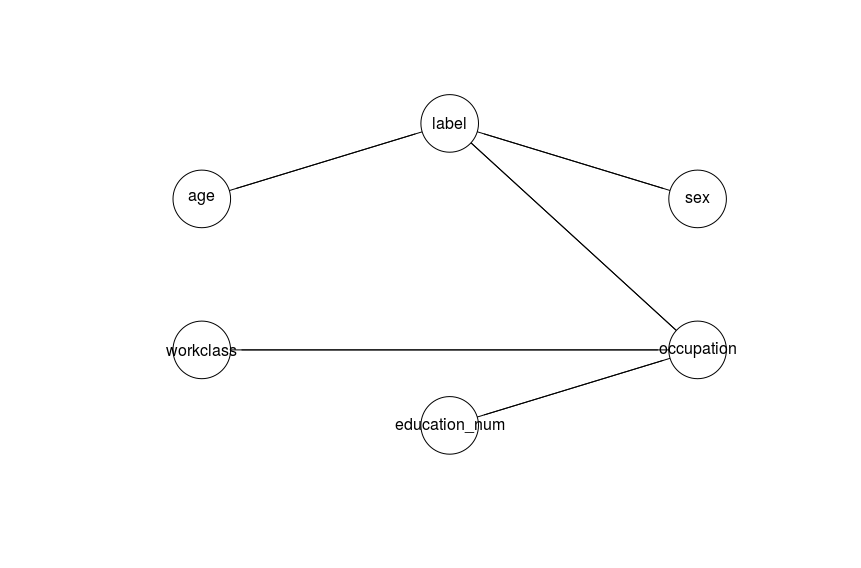
\includegraphics[width=.9\linewidth]{./img/net_cl.png}
\caption{Network learned using Chow-Liu}
\end{figure}

\begin{figure}[htb]
\centering
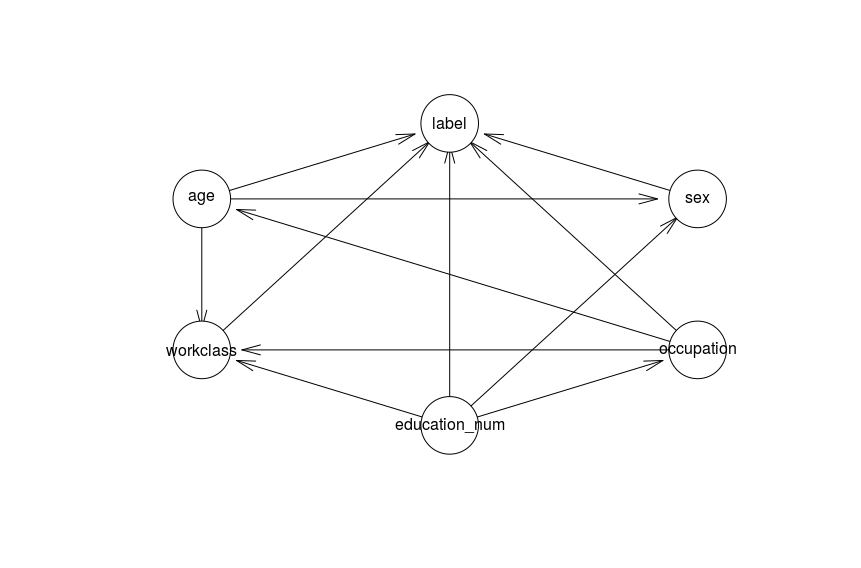
\includegraphics[width=.9\linewidth]{./img/net_hc.png}
\caption{Network learned using Hill-Climbing}
\end{figure}

From the code above, we get the two structures shown in Figure 1 and Figure 2. We can see that
the structure learned by Chow-Liu is much more interesting and similiar to the one we expected.
Hill-Climbing ended up representing too many connections (dependencies), which makes the graph
too complex for the kind of problem we are trying to represent. For this reason, we select the
network generated by Chow-Liu to be the one we are going to fit and try to learn the parameters.

Something we should do before that, tough, is to transform the acyclic graph into a cyclic
one. Selecting the label as the root of our tree, it is now simple to decide for a direction for
all arcs:

\begin{figure}[htb]
\centering
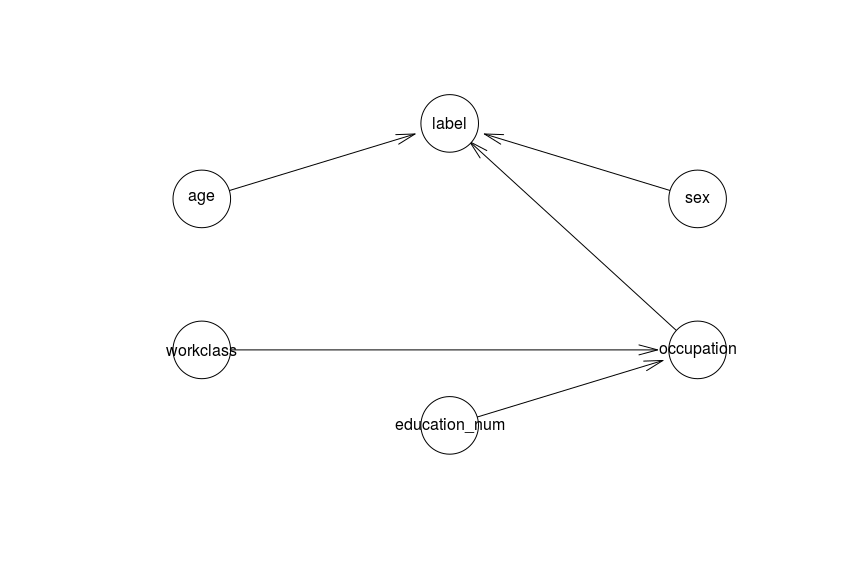
\includegraphics[width=.9\linewidth]{./img/net_cl_dir.png}
\caption{Our learned network with directed arcs}
\end{figure}

From Figure 3, we see that the network learned by our method is different from the one we were
expecting: 
% Emacs 24.5.1 (Org mode 8.2.10)
\end{document}
